\documentclass[a4paper,11pt]{article}
\usepackage{ctex}
\usepackage{fancyhdr}
\usepackage{graphicx}
\usepackage{float}
\usepackage{geometry}
\usepackage{amsmath}
\usepackage{enumerate}
\usepackage{amstext}

\geometry{left=2.0cm, right=2.0cm, top = 3cm, bottom=3cm}
\pagestyle{fancy}
\fancyhf{}
\lhead{\leftmark}
\rhead{\rightmark}
\cfoot{\thepage}
\newcommand*{\dif}{\mathop{}\!\mathrm{d}}
\newcommand*{\e}{\mathop{}\!\mathrm{e}}

\title{弦振动实验}
\author{左京伟 \qquad 未央-电11 \qquad 2021012328}
\date{\today}


\begin{document}
\maketitle
\begin{abstract}
    本实验的原理主要包括:波动方程的推导和应用,波的反射和叠加原理以及驻波的条件与性质。实验主要内容为:了解振动在弦线上的传播现象,学习弦振动方程,分析弦末端固定时的边界条件和反射特性,以及观察和测试弦线在周期性正弦激励下的受迫振动(尤其是驻波)现象,最后利用示波器测量共振频率,用直线拟合的方式探究影响振动频率的因素。
\end{abstract}

\section{实验仪器}
    6根直径不同的弦线,线密度如图\ref{fig:弦线的线密度}。\\
    \begin{figure}[ht]
        \centering
        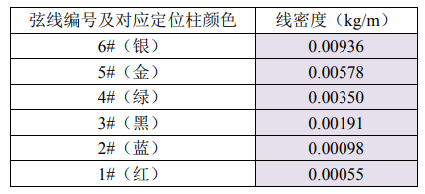
\includegraphics[scale=0.7]{弦线的线密度.png}
        \caption{弦线的线密度}
        \label{fig:弦线的线密度}
    \end{figure}

    \begin{figure}[ht]
        \centering
        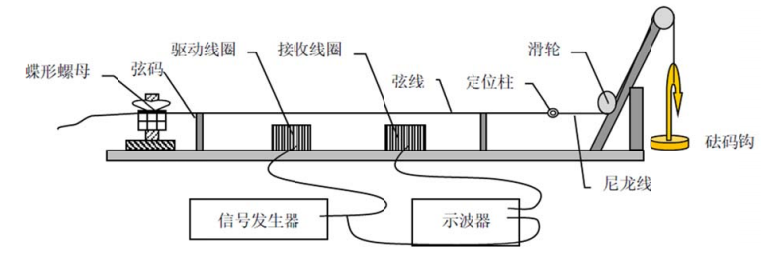
\includegraphics[scale=0.6]{实验设备.png}
        \caption{实验装置}
        \label{fig:实验设备}
    \end{figure}

    砝码钩1个,砝码5个,质量均为200g(用来改变弦线上的张力)

    底座1个,包含蝶形螺母(用来固定弦线)、两个弦码(作为反射面),滑轮和底部的驱动线圈(提供周期激励)和接收线圈(测量弦线振动频率)。

    信号发生器与示波器,分别连接驱动线圈和接受线圈。

    实验装置的摆放如图\ref{fig:实验设备}。

    注意点:
    \begin{enumerate} [i.]
        \setlength{\itemindent}{2em}
        \item 发射线圈和接受线圈之间的距离不要太短($>10$cm),以免互感现象干扰对振动波形的观测。
        \item 驱动线圈和接受线圈与弦码之间的距离都要$>5$cm。
        \item 驱动线圈和接受线圈尽量都要放置在波腹左右的位置上,这样方便观测波形。
    \end{enumerate}

\section{实验内容}
    \subsection{理论部分}
        \subsubsection{弦振动方程}
            下面我们来推导匀质软绳上的横波的振动方程。

            假设有一根半无限长,沿着$+x$轴放置的柔软均匀的弦线被拉紧,弦线中张力为$T$。\footnote{如何给半无限长的绳子施加张力?这里所谓“无限”,其实是一种绳长远大于波长的等价表述。本实验中测量的是绳形成的驻波,而驻波可以看成是两个相反方向的无限长绳振动的叠加,所以不会有逻辑漏洞。}在弦线的始端$x=0$处加以$y$方向的振动激励之后,由于弦线中的张力作用,弦线的振动形式将会随着绳子传播。

            对位于$(x, x+\dif x)$上的一小段弦线进行受力分析,如图\ref{fig:弦线受力分析}所示。

            \begin{figure}[ht]
                \centering
                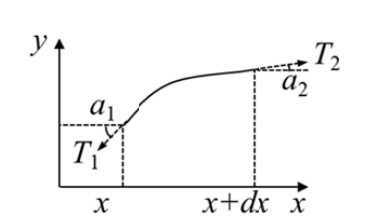
\includegraphics[scale=0.7]{弦线受力分析.png}
                \caption{弦线受力分析}
                \label{fig:弦线受力分析}
            \end{figure}

            由于弦线没有水平方向上的位移,因此$\dfrac{\partial x}{\partial t} \equiv 0$,下面仅对$y$列出运动学方程。

            水平方向受力平衡
            \begin{equation}
                T_2\cos\alpha_2 - T_1\cos\alpha_1 = 0
                \label{x}
            \end{equation}

            竖直方向的牛二方程,其中已设绳的线密度为$\rho$
            \begin{equation}
                T_2\sin\alpha_2 - T_1\sin\alpha_1 = \rho\dif x \frac{\partial^2 y}{\partial t ^2}
                \label{y}
            \end{equation}
            当振动幅度很小,即$\alpha \approx 0$时,有近似条件$\sin\alpha_1 \approx \tan \alpha_1 = \dfrac{\partial y}{\partial x}\bigg|_x $,$\sin\alpha_2 \approx \tan \alpha_2 = \dfrac{\partial y}{\partial x}\bigg|_x +\dif x$,以及$\cos\alpha_1,\cos\alpha_2 \approx 1$,代入 式(\ref{x})和 式(\ref{y})得
            \begin{equation}
                T_1 \approx T_2 \approx T
            \end{equation}

            \begin{equation}
                \dfrac{\partial^2y}{\partial t^2} - \dfrac{T}{\rho} \dfrac{\partial^2y}{\partial x^2} = 0 
                \label{wave eqn}
            \end{equation}
            由此易得波速为
            \begin{equation}
                v = \sqrt{\dfrac{T}{\rho}}
                \label{v}
            \end{equation}
            式(\ref{wave eqn})的通解为$f(vt \pm x)$,其中负号代表波向$+x$方向传播的方程,正号代表波向$-x$方向传播的方程。\footnote{一个简单的判断方法是,看过了一段时间(即$t>0$)之后,波传播到的位置,即$f(0)$将在哪一个$x$处获得。当括号中是正号时,$x$是一个负值,而负号时$x$为正值。}

            又由式(\ref{v})知,弦振动波形传递的波速$v$仅仅和弦上张力$T$和弦线线密度$\rho$有关。
        
        \subsubsection{弦线末端固定时的边界条件及反射现象}

            \begin{figure}[ht]
                \centering
                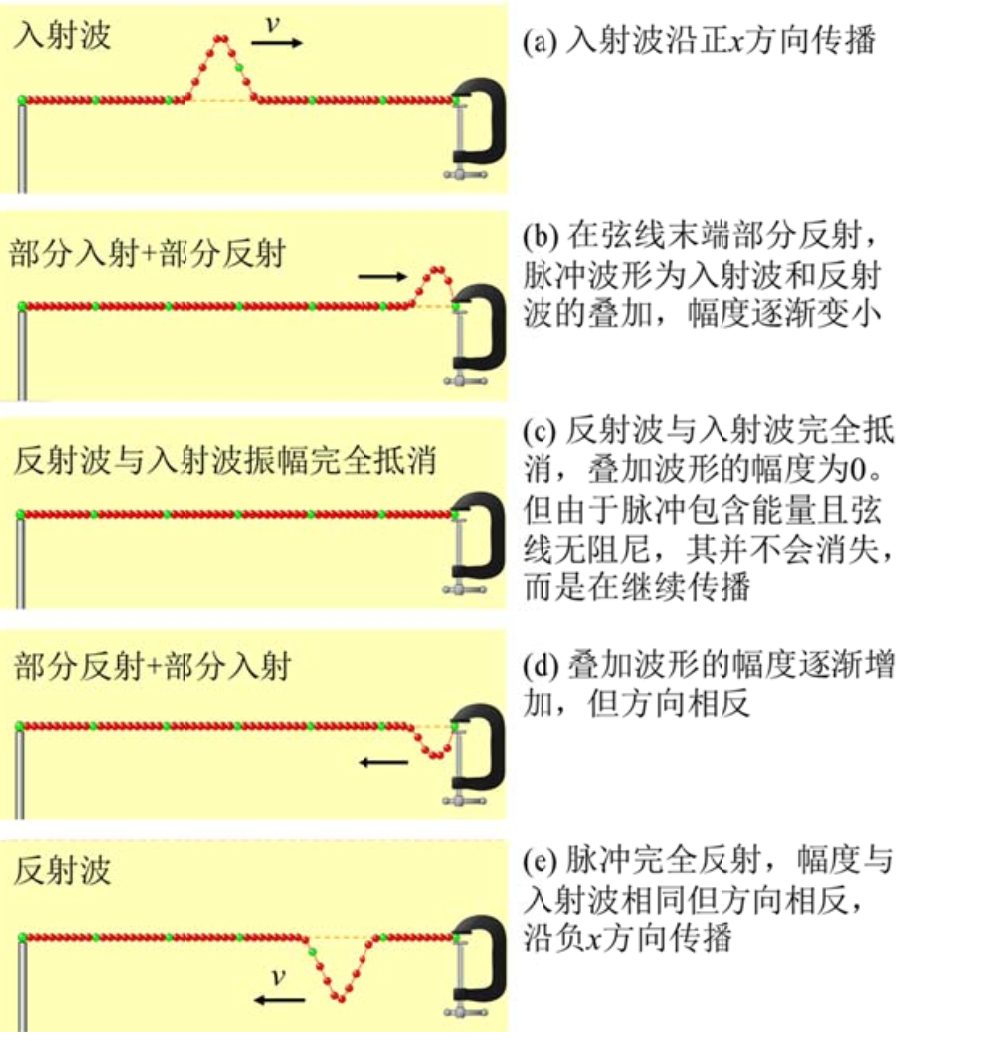
\includegraphics[scale=0.7]{反射.png}
                \caption{弦末端固定时脉冲的反射及其与入射波的干涉(叠加)现象}
                \label{反射}
            \end{figure}
            
            因为这里是完全固定的状态,为了保证右端点处位移恒为零,反射波必然在右端点处的振动位移和入射波完全抵消,即$y_{in}(vt-x)\big|_{x=L} \equiv y_{reflect}(vt+x)\big|_{x=L}$,因此反射系数$R = 1$。
            
        \subsubsection{弦线在周期性正弦激励下的受迫振动和共振(或驻波)现象}

            下面分析,在周期性正弦激励下,弦线形成共振(驻波)的条件。

            设弦线上沿着$+x$方向传播的波为$y^+ = A^+ \e^{i(\omega t-kx+\varphi^+)}$,\footnote{复数表示振动。由欧拉公式$e^{i\theta} = \cos\theta + i\sin\theta$。}沿着$-x$方向传播的波为$y^- = A^- \e^{i(\omega t+kx+\varphi^-)}$。则合振动为\footnote{由于波的叠加原理。}

            \begin{equation}
                y=A^+ \e^{i(\omega t-kx+\varphi^+)} + A^- \e^{i(\omega t+kx+\varphi^-)}
                \label{sum}
            \end{equation}

            波的边界条件为弦线两端固定,即$y(t,x=0)=0$与$y(t,x=L)=0$。得到
            
            \begin{equation}
                A^- = -A^+ \e^{i(\varphi^+-\varphi^-)}
            \end{equation}

            回代入式(\ref{sum})得到

            \begin{equation}
                y = -2A^+\e^{i\varphi^+}\sin kx \e^{i\omega t}
                \label{final y}
            \end{equation}

            令初相位$\varphi^+ = 0$,并且取实部得到
            
            \begin{equation}
                y = -2 A^+ \sin kx\cos \omega t 
            \end{equation}

            可以发现,形成驻波时,弦上每处都在做简谐振动,振幅仅与$x$有关,为$|2A^+\sin kx|$.
            
            难道说只要弦的两端被固定,就一定会形成驻波吗?未必。下面探讨何时驻波形成的条件。

            将边界条件$y(t,x=L)=0$代入式(\ref{final y})可知,驻波形成的条件为$\sin kL = 0$,也即$\dfrac{2\pi}\lambda L = n\pi$,或$l=n\dfrac\lambda 2$,其中$n$为自然数。所以,弦上形成驻波的条件是弦长$L$为半波长$\dfrac\lambda 2$的整数倍。\footnote{在测量中,如何判断形成了驻波呢?实际只需要观察到振动的波形稳定最大即可。因为如果弦上没有形成驻波,会有类似“拍”的振荡形式,即波形会一边振动一边平移,而且振幅会比驻波的情形小。}

            \begin{figure}[ht]
                \centering
                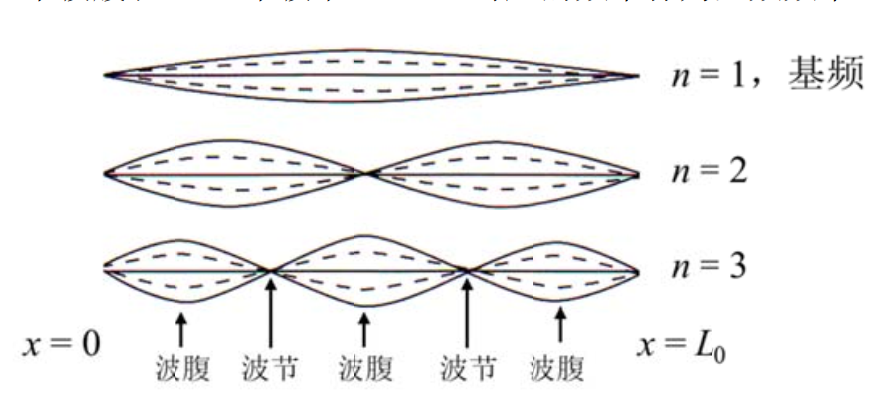
\includegraphics[scale=0.7]{驻波.png}
                \caption{驻波的波形示意图}
                \label{驻波}
            \end{figure}

            形成驻波之后,波形看起来就像昆虫的身体。最宽(也即振幅最大)的地方称作“波腹”,窄的地方(振幅为0的地方)称作“波节”。$n$次谐频有$n$个波腹和$n-1$个波节。$n=1$对应的频率称为基频频率。

            由$v=f\lambda$,还可以得到驻波频率和弦线参数的关系

            \begin{equation}
                f = \dfrac{n}{2L} v = \dfrac{n}{2L}\sqrt{\dfrac{T}{\rho}}
                \label{freq}
            \end{equation}

        \subsection{实验部分}

            从式(\ref{freq})可知,弦振动频率和$n$、$L$、$T$、$\rho$有关。下面采取控制变量的方法,分别研究这4个影响因素。本实验中肿瘤加速度$g$均取9.80m/s。

            \subsubsection{观察弦振动,分析$f\sim n$关系}

                选用粗弦6\#银弦,在弦长$L=50.0cm$,张力$T=9.80$N的条件下,用信号发生器产生合适频率的激励,观察弦振动现象。在$n=$1、2、3、4、5的驻波情况下,测量共振频率,并且使用最小二乘法对$f$、$n$进行直线拟合。数据如图(\ref{data1})所示。

                \begin{figure}[ht]
                    \centering
                    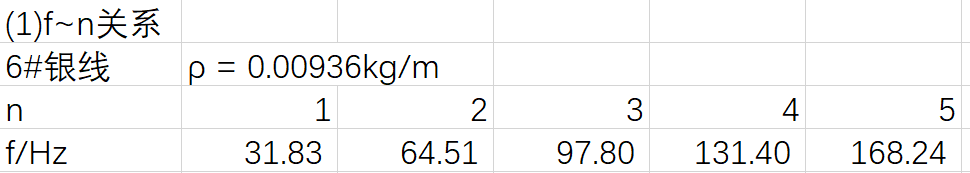
\includegraphics[scale=0.7]{1.f~n关系.png}
                    \caption{$f\sim n$关系}
                    \label{data1}
                \end{figure}

                由Excel表格拟合得出斜率的测量值为$$k=33.11~s^{-1}$$

                并经过计算得到不确定度\footnote{这里的自由度$\nu$取$n-1$,因为这是一条过原点的直线,2.2.2中也是如此。但是2.2.3及2.2.4的拟合当中,由于直线不过原点,所以自由度$\nu$取$n-2$,特此说明,在后续小节不再另行脚注。}$$U_k = s_k \cdot tinv(1-0.95, 5-1) = 0.263033873 \times 2.776445105
                = 0.730299108~s^{-1}$$

                因此斜率测量结果为$$k = (33.1 \pm 0.7)~s^{-1}$$

                根据式(\ref{freq})得到,$f\sim n$直线理论的斜率为

                $$k' = \dfrac{1}{2L}\sqrt{\dfrac{T}{\rho}} = \dfrac{1}{2\times 0.5000\text{m}}\sqrt{\dfrac{\text{9.80N}}{\text{0.00936kg/m}}} = 32.4~s^{-1}$$

                实际测得斜率和理论值的相对误差为\footnote{经过初步分析,笔者认为误差来源可能为读取谐振频率时,由于需要手动调节信号发生器的发射频率,观察输出波形是否达到稳定的最大,存在一定的\textbf{主观因素}影响。当输出频率和共振频率接近时,共振波形在极其缓慢地上下浮动,左右漂移,由于时间尺度过大,很难真正使得测量得到的频率数据误差在仪器误差限以内。这种误差来源广泛存在于本次实验的所有频率读取过程当中。}$$\varepsilon_k = \dfrac{k-k'}{k'} = \dfrac{33.1-32.4}{32.4} = 2.16\%$$

            \subsubsection{分析$f\sim L$关系}

                选用中粗弦3\#黑弦,在张力$T=9.80$N的条件下,用信号发生器产生合适频率的激励,观察弦振动现象。在形成$n=1$的驻波情况下,从30.0cm到55.0cm范围内每间隔5.0cm改变弦长L,测量相应的共振频率$f$,并且使用最小二乘法对$f$、$\dfrac 1L$进行直线拟合。数据如图(\ref{data2})所示。

                \begin{figure}[ht]
                    \centering
                    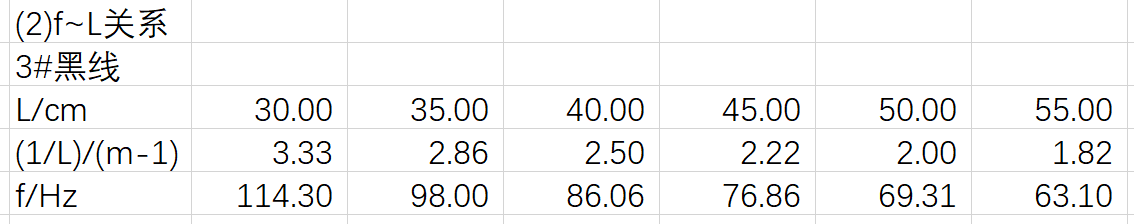
\includegraphics[scale=0.7]{2.f~L关系.png}
                    \caption{$f\sim L$关系}
                    \label{data2}
                \end{figure}

                由Excel表格拟合得出斜率的测量值为$$k=34.42814976~\text{m/s}$$

                并经过计算得到不确定度$$U_k = s_k \cdot tinv(1-0.95, 6-1) = 0.070178663 \times 2.570581836 = 0.180399997~\text{m/s}$$

                因此斜率测量结果为$$k = (34.43 \pm 0.18)~\text{m/s}$$

                根据式(\ref{freq})得到,$f\sim \dfrac 1L$直线理论的斜率为

                $$k' = \dfrac{n}{2}\sqrt{\dfrac{T}{\rho}} = \dfrac{1}{2}\sqrt{\dfrac{\text{9.80N}}{\text{0.00191kg/m}}} = 35.82~\text{m/s}$$

                实际测得斜率和理论值的相对误差为$$\varepsilon_k = \dfrac{k-k'}{k'} = \dfrac{34.43-35.82}{35.82} = -3.88\%$$

            \subsubsection{分析$f\sim T$关系}

                选用细弦1\#黑弦,保持$L=50.00$cm不变,在1.96N到11.76N之间改变弦上张力,在形成$n=1$的驻波情况下,测量相应的共振频率$f$,并且使用最小二乘法对$\ln f$、$\ln T$进行直线拟合。数据如图(\ref{data3})所示。
                
                \begin{figure}[ht]
                    \centering
                    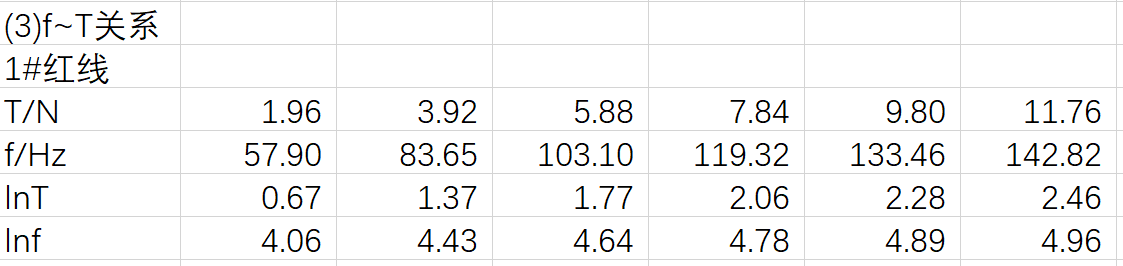
\includegraphics[scale=0.7]{3.f~T关系.png}
                    \caption{$f\sim T$关系}
                    \label{data3}
                \end{figure}
                
                由Excel表格拟合得出斜率的测量值为$$k=0.50936177$$

                并经过计算得到不确定度$$U_k = s_k \cdot tinv(1-0.95, 6-2) = 0.008548257 \times 2.776445105 = 0.023733767$$

                因此斜率测量结果为$$k = 0.509 \pm 0.024$$

                根据式(\ref{freq})得到,$\ln f\sim \ln T$直线理论的斜率为

                $$k' = \dfrac 12 = 0.500$$

                实际测得斜率和理论值的相对误差为$$\varepsilon_k = \dfrac{k-k'}{k'} = \dfrac{0.509-0.500}{0.500} = 1.80\%$$

            \subsubsection{分析$f\sim \rho$关系}
                
                保持$L=50.00cm$,$T=9.80N$不变,分别测量1\#到6\#弦的基频($n=1$)共振频率,测量相应的基频频率$f$,并且使用最小二乘法对$\ln f$、$\ln \rho$进行直线拟合。数据如图(\ref{data3})所示。
                
                \begin{figure}[ht]
                    \centering
                    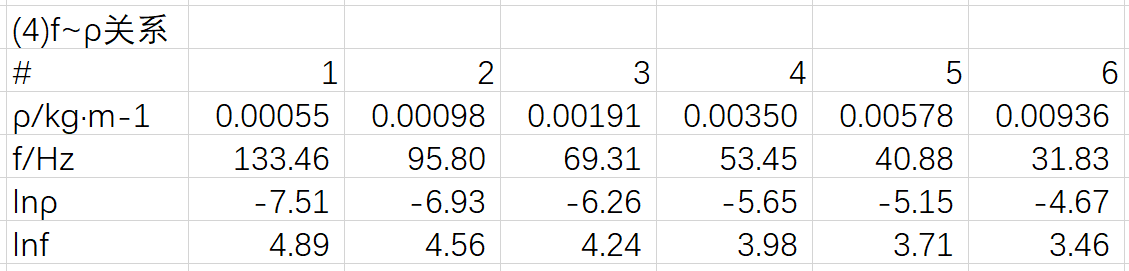
\includegraphics[scale=0.7]{4.f~ρ关系.png}
                    \caption{$f\sim \rho$关系}
                    \label{data4}
                \end{figure}
                
                由Excel表格拟合得出斜率的测量值为$$k=-0.496271722$$

                并经过计算得到不确定度$$U_k = s_k \cdot tinv(1-0.95, 6-2) = 0.009126232 \times 2.776445105 = 0.025338482$$

                因此斜率测量结果为$$k = -0.496 \pm 0.025$$

                根据式(\ref{freq})得到,$\ln f\sim \ln T$直线理论的斜率为

                $$k' = \dfrac 12 = -0.500$$

                实际测得斜率和理论值的相对误差为$$\varepsilon_k = \dfrac{k-k'}{k'} = \dfrac{-0.496- (-0.500)}{-0.500} = 0.80\%$$

            \subsubsection{分析弦的线密度、弦长、张力、基频与波速的关系}

                这里控制绳上张力不变,选取不同线密度的弦线,分别计算波速,并与理论波速相比较。实验数据如图(\ref{波速})所示。

                \begin{figure}[ht]
                    \centering
                    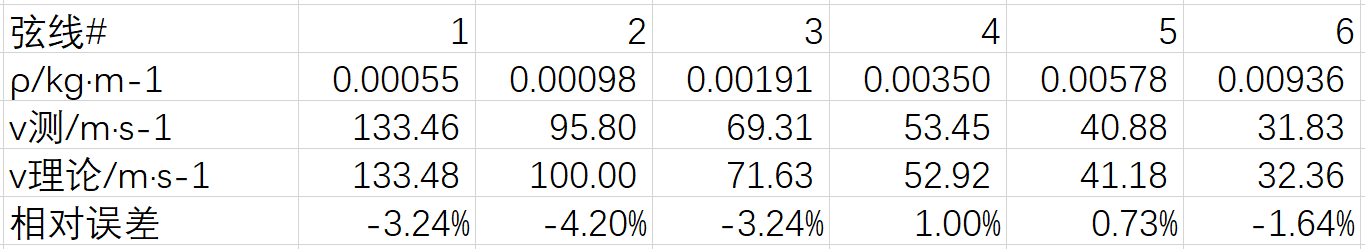
\includegraphics[scale=0.7]{波速.png}
                    \caption{波速数据}
                    \label{波速}
                \end{figure}

                其中实验测得的波速为$$v = f\lambda = \dfrac{2L}{n}f$$

                选取$n=1$,即可计算得到图(\ref{波速})中第三行的数据。

                理论的波速计算方式为$$v'=\sqrt{\dfrac{T}{\rho}}$$

                相对误差为$$\varepsilon =\dfrac{v-v'}{v'}$$

                由上两式,计算得到图(\ref{波速})中第四、五两行的数据。可以发现误差还是有一些大的,初步分析判断,除了之前提到的读取频率的人差之外,还有可能是因为弦线密度和基准值有偏差。因为弦线重复用了很多次,承受拉力的时间长了之后,会有绳长方向的延展,造成线密度降低,所以理论值会偏大。这种判断也和相对误差总是小于0的事实相符合。

            \subsubsection{激励线圈和探测线圈放置的位置}
                参见“实验仪器”一节中最后的三个注意点(i. ii. iii.),此处不再重复。
            \subsubsection{快速找到弦振动的共振频率的方法}
                首先,计算得出当前共振频率的理论值,将信号发生器调节到理论值附近,调节步长设置为1Hz,先粗调。找到波形变化比较缓慢的频率附近\footnote{当频率接近共振频率时,会形成拍振,波形发生缓慢横向移动,当激励频率高于共振频率时和低于共振频率时,拍的位移方向相反。由此可以断定,当调节1个步长之后,拍的漂移方向反转时,共振频率即处在这两个频率之间。},再将步长设置为0.1Hz,继续调节,再进而设置步长为0.01Hz,重复上述过程,直到看到的输出波形为振幅最大的稳定正弦波为止。
\section{分析讨论}
    \begin{enumerate}[i.]
        \item 实验时要注意弦线的尾端位置,不要让砝码钩和任何物体有接触,否则绳上张力会有偏差。
        \item 实验中的误差来源主要是弦线线密度实际会偏小;共振频率读数有人差;在多次改变张力测量弦线共振频率时,弦线的长度会有些微拉伸,造成弦码的微小位移,这往往容易被实验者忽略。
        \item 其余一些细碎的讨论,均已以脚注的形式随文附上。
    \end{enumerate}

\section*{附录:原始数据}

    第(3)点中把最右侧的频率值划去的原因是,一开始测的这个数据,发现砝码和底座有接触,造成拉力不准,后来更改砝码位置重新测量。

    第(5)点划去的原因是,一开始以为只要选取一个数据测量波速。后来经过老师的提醒发现这样不具有代表性,因此增加了其他数据,画成一张表格在下方。

    \begin{figure}[ht]
        \centering
        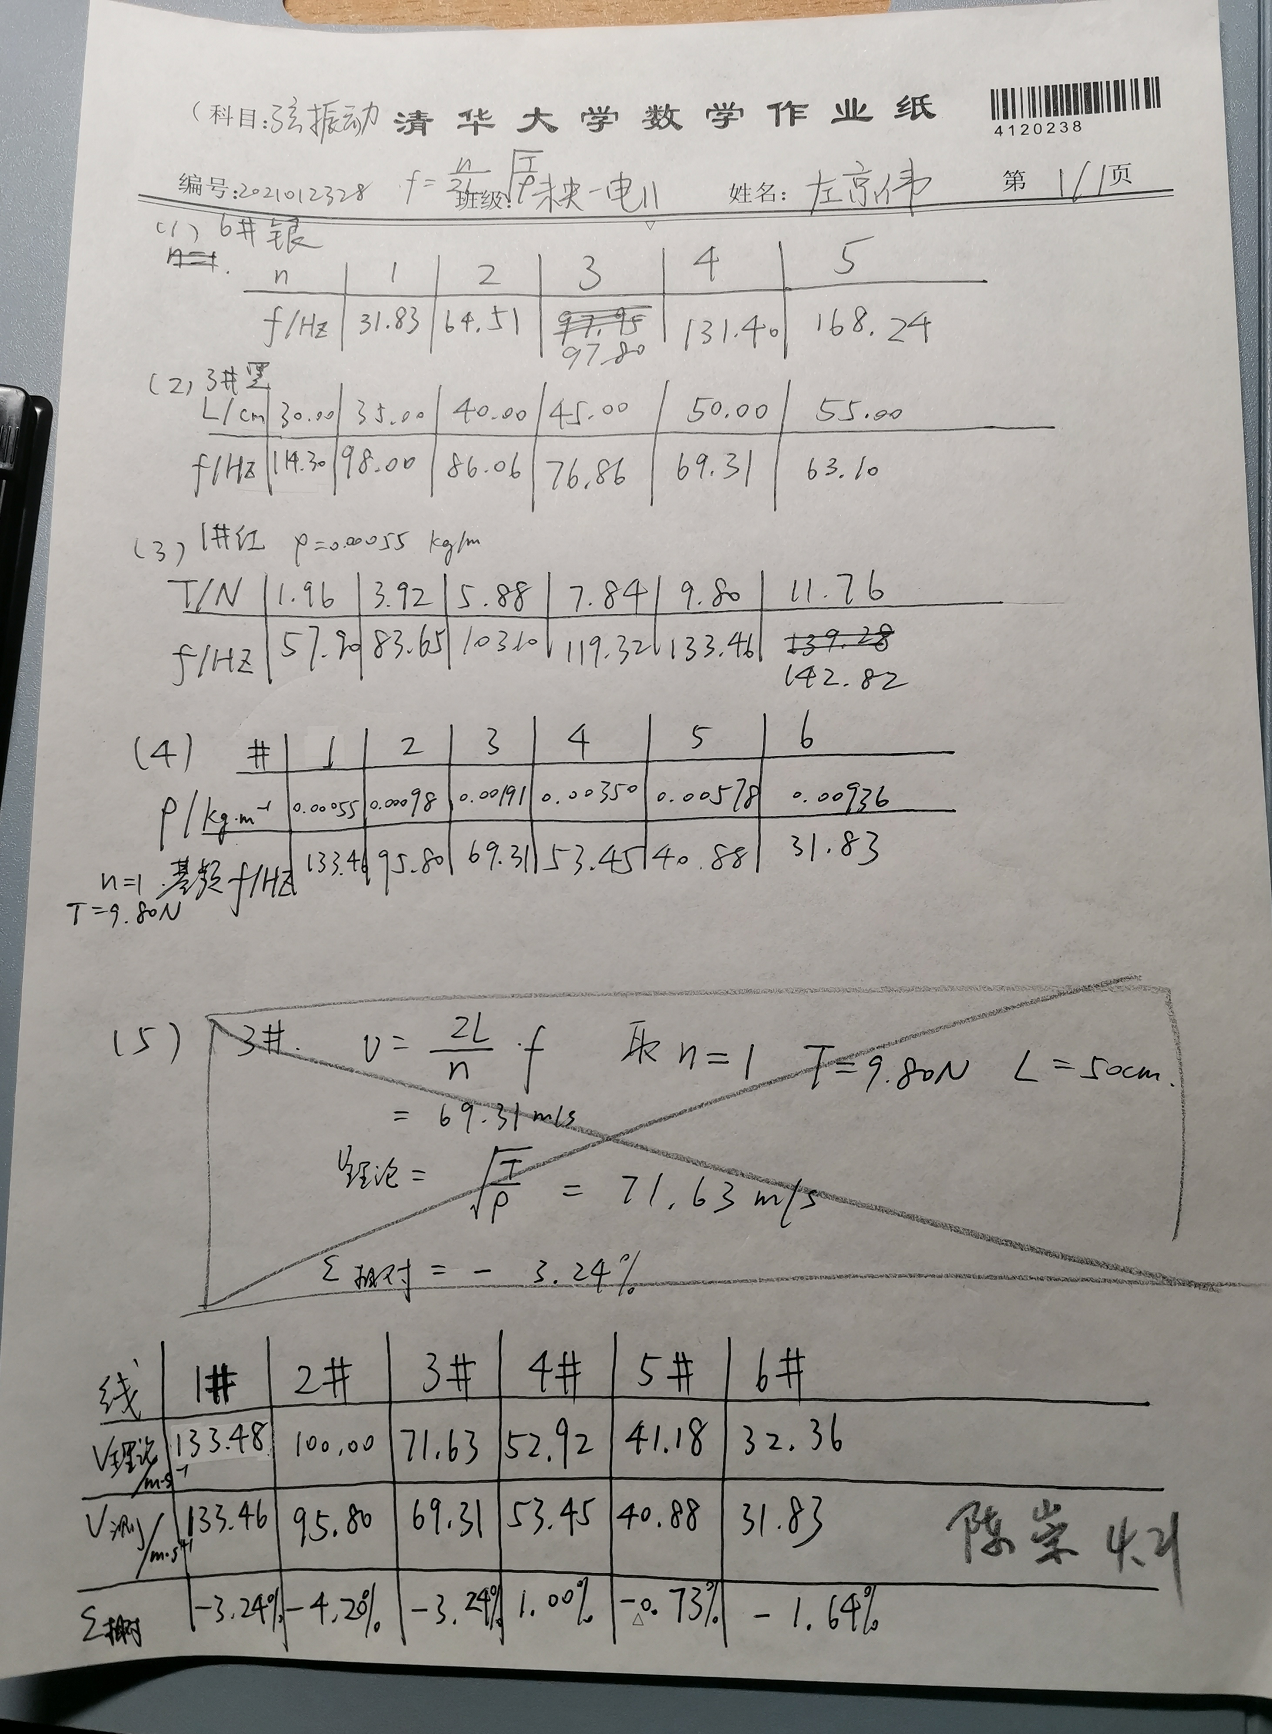
\includegraphics[scale=0.6]{原始数据.png}
        \caption{原始数据}
        \label{fig:label}
    \end{figure}

\end{document}